\chapter{Reinforcement Learning and Deep Neural Networks}
\label{ch:reinforcement_learning}

\begin{remark}{Outline}

\end{remark}

\section{Introduction}
\label{sec:rl_introduction}


\section{Markov Decision Processes}
\label{sec:mdps}

In order to develop and apply RL algorithms to optimal decision making problems, we need to formulate the problem in a specific framework: in RL this is done with Markov Decision Processes (MDPs). Throughout this thesis we will characterize MDPs, and the resulting RL concepts, by using the mathematical notation that was used by \citet{sutton2018reinforcement} in their seminal book about RL, although it is worth noting that within the literature, different formulations can be found to express the same kind of concepts \cite{busoniu2010reinforcement}.

We start by introducing the following elements:
\begin{itemize}
	\item A set of possible states $\mathcal{S}$, that can be visited by an agent while it is interacting with the MDP, where $s_t \in \mathcal{S}$ denotes the state being visited at time-step $t$.
	\item A set of possible actions $\mathcal{A}$ that are available to the agent when it is in a certain state, where $a_t \in \mathcal{A}(s_t)$ denotes the action that is performed by the agent in state $s$ at time-step $t$.
\item A transition function $\mathcal{P}:\matchal{S}\times\matchal{A}\times\matchal{S}\Rightarrow [0,1]$ that defines the probability for an agent to visit state $s_{t+1}$, based on its current state and the action which will be performed thereafter.
\item A reward function $\Re:\matchal{S}\times\matchal{A}\times\matchal{S}\Rightarrow \mathbb{R}$ which returns a reward signal $r_{t+1}$ when an agent performs action $a_t$ in state $s_t$ and transits to $s_{t+1}$.
\item A discount factor denoted as $\gamma \in [0,1]$.

\end{itemize}

Based on these concepts a MDP is then defined by the following tuple $<\mathcal{S}, \matchcal{A}, \matchal{P}, \Re, \gamma>$ and is also commonly denoted in the RL literature as the \textcolor{RoyalBlue}{environment}. The way the agent interacts with this environment is given by its \textcolor{RoyalBlue}{policy} $\pi$, defined as a probability distribution over $a \in \matchal{A}(s)$ for each $s \in \mathcal{S}$:
\begin{equation}
	\pi(a|s) = \text{Pr}\; \{A_t = a | S_t = s\}, \; \text{for all}\; s \in \mathcal{S}\; \text{and}\; a\ \in \mathcal{A}. 
\end{equation}
A policy can be deterministic if $\forall s:\pi(s,a) = 1$ for exactly one $a \in \mathcal{A}(s)$ and $\pi(s,b)=0$ for all other $b \in \mathcal{A}(s)$, while it is stationary if it does not change over time. In both cases the goal of a policy is to map each state to an action $\pi:\mathcal{S}\Rightarrow\mathcal{A}$.

The elements of a MDP allow us to properly model the dynamics of an agent interacting with its environment, an interaction which can be summarized as follows: at each time-step $t$ the environment provides the agent with a certain state $s_t$, the agent then performs action $a_t$ which results into the reward signal $r_{t+1}$. After performing such action the agent will enter into a new state $s_{t+1}$. This continuous interaction with the environment is also known as the Reinforcement Learning loop, and can technically be infinite. This is however never the case in practice, since an agent will eventually visit a state which only transits to itself (denoted as terminal), which will therefore stop the agent-environment interaction. We visually represent the Reinforcement Learning loop in Fig. \ref{fig:rl_loop}.

\begin{figure}[ht!]
\centering
  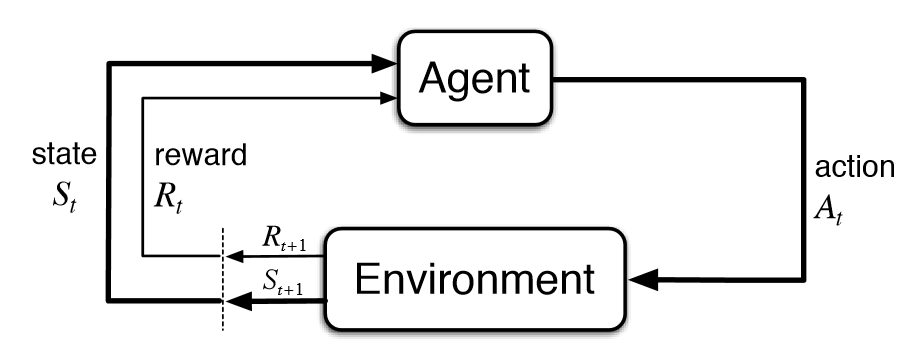
\includegraphics[width=10cm]{./Images/Chapter06/rl_loop.png}
  \caption{A visual representation of how an agent interacts with an environment as modeled by a Markov decision process. Figure taken from page 48 of the \citet{sutton2018reinforcement} textbook.}
  \label{fig:rl_loop}
\end{figure}

Each interaction of the agent with the environment is defined as an \textcolor{RoyalBlue}{episode}, which consists of one, or several trajectories $\tau$, that come in the form of the following sequence:
\begin{align}
	\langle(s_t,a_t,r_t,s_{t+1})\rangle,t=0,\ldots,T-1
\end{align}
where $T$ is a random variable representing the length of the episode.

A key property of the environment is that it fulfills the Markov property which is defined as follows:
\begin{definition}
	A discrete stochastic process has the Markov property if the conditional distribution of the next state of the process only depends from the current state of the process.
\end{definition}
This implies that the only information that is necessary for predicting to which state an agent will step next are $s_t$ and $a_t$, which can be expressed formally as:
\begin{align}
	p(s_{t+1}|s_t, a_t, s_{t-1}, a_{t-1}, \ldots) = p(s_{t+1} | s_t, a_t).
\end{align}
Interestingly, a similar conclusion also holds for the reward that the agent will get, meaning that the reward that is obtained by an agent is only determined by its previous action, and not by the history of all previously taken actions, as defined by:
\begin{align}
	(r_t| s_t, a_t, \ldots, s_1, a_1) = p(r_t|s_t,a_t).
\end{align}

\section{Goals and Returns}
So far we have defined all the elements that model the interaction of an agent with an environment, whilst introducing some key properties that are key for the development of RL algorithms. While it is true that we have defined how the agent-environment interaction works, we yet do not know what the purpose of this interaction is. In RL the goal of an agent is defined with respect to the reward signal $r_t$ that is returned by the reward function $\Re$. Informally, the goal of an agent is that of maximizing the total amount of reward it receives while interacting with the environment. In the simplest case we can define this as:
\begin{align}
	G_t = r_t, r_{t+1}, r_{t+2}, \ldots, r_{T}.
\label{eq:goal}
\end{align}
While simple and intuitive this formulation has one major drawback: it treats each reward signal equally since it does not distinguish rewards that are obtained in the near future, i.e. $r_t$, from the ones that will be obtained in the more distant future, i.e. $r_{T-1}$. To deal with such issue we need an additional concept known as \textcolor{RoyalBlue}{discounting}, which can be governed by the discount rate parameter $\gamma$, also known as the discount factor. $\gamma$ allows us to weight the different reward signals based on how close or distant in the future these rewards are received by the agent. By introducing $\gamma$ in Eq. \ref{eq:goal} we can now define the expected discounted return as:
\begin{align}
	G_t & = r_t+\gamma r_{t+1}, \gamma^{2} r_{t+2} + ... \\
	    & = \sum_{k-0}^{\infty}\gamma^{k} r_{t+k+1}.
\label{eq:discounted_return}
\end{align}
The role of $\gamma$ can be interpreted as follows: a reward obtained $k$ time steps in the future is only worth $\gamma^{k-1}$ times what it would be worth if received immediately. It is easy to see how different $\gamma$ values can result into different agent's behaviors. If $\gamma=0$ an agent will only take into account immediate rewards, therefore aiming to maximize $r_{t+1}$ only and resulting into having a ``myopic" behavior. If $\gamma$ approaches $1$ the agent will become more ``far-sighted", it will take future rewards into account more strongly and will therefore increase its chances of accessing future rewards that will result into a higher cumulative return. 
Please note that by defining $\gamma \leq 1$ we can make the infinite sum presented in Eq. \ref{eq:discounted_return} finite as long as the sequence of rewards $r_k$ is bounded.   

While the role of $\gamma$ is often taken for granted within the RL literature it is worth noting that as mentioned by \citet{van2011insights} and \citet{schmidhuber2019reinforcement}, $\gamma$ is an artificial concept which is not present in fields such as traditional control theory or engineering. The reason of this is that $\gamma$ corresponds to a concept that does not exists in the real world, and that in practice distorts the real value of $r_t$ in an exponentially shrinking fashion. Even if it is considered common practice to include a discount factor in the development of RL algorithms, it is worth noting that making $\gamma$ part of the RL framework corresponds to including a form of ``inductive bias" within the resulting algorithms. It is common knowledge that low discount factors result into poor performance, and that it is therefore as beneficial as possible to set $\gamma$ as close to $1$, yet choosing an appropriate $\gamma$ parameter can be more challenging than expected especially when RL algorithms are combined with function approximators. \citet{wiering2009qv} show that different algorithms prefer different discount factors, while \citet{franccois2015discount} show the relationship between low discount factors and the values of the learning rate. Finally \citet{van2019using} introduce a method that allows the use of low discount factors for approximate RL algorithms, while at the same time highlighting that the common perception of the role of $\gamma$ might need revision from the RL community.             

\section{Value Functions}
We are now ready to introduce the arguably most important concept that underlies many RL algorithms: the concept of \textcolor{RoyalBlue}{value}. We can define the value of a state $s$, as well as the value of a certain policy $\pi$ or of a certain action $a$, anyhow, independently from what we are considering the notion of value is always directly linked to the concept of expected discounted return defined in Eq. \ref{eq:discounted_return}. Given an MDP and a policy $\pi$ we can determine the value of a state $s$ as a function that measures the expected return that the agent will receive when starting in $s$ and following $\pi$ thereafter. 
\begin{align}
    V^{\pi}(s)=\mathds{E}\bigg[\sum_{k=0}^{\infty}\gamma^{k}r_{t+k}\bigg| s_t = s, \pi \bigg].
    \label{eq:state_value_function}
\end{align}
$V^{\pi}(s)$ is also known as the \textit{state-value function} and intuitively tells us how good or how bad it is for an agent to be in a certain state. While this function is only conditioned on the state that is being visited by the agent, we can also condition it on the actions that are taken by the agent, which will measure how good or bad it is for the agent to take a certain action $a$ in a certain state. This function comes with the name of \textit{state-action value function} and is defined as follows:
\begin{align}
     Q^{\pi}(s,a)=\mathds{E}\bigg[\sum_{k=0}^{\infty}\gamma^{k}r_{t+k} \bigg| s_t = s, a_t=a, \pi\bigg].
 \end{align}
Both value functions are very powerful since they allow us to characterize the behavior of an agent by quantitatively assessing its interaction with the environment. They can be seen as the knowledge of the agent and represent its desirability of being in a specific state.   

In RL we are interested in maximizing the value of each state or of each state-action pair, since by doing so we will be finding an optimal policy $\pi^{*}$ that realizes the optimal expected return defined as:
\begin{align}
 V^{*}(s)=\underset{\pi}{\max}\:V^{\pi}(s), \ \text{for all} \ s\in\mathcal{S}
\end{align}
and the optimal $Q$ value function:
\begin{align}
Q^{*}(s,a)= \underset{\pi}{\max}\:Q^{\pi}(s,a) \ \text{for all} \ s\in\mathcal{S} \ \text{and} \ a \in\mathcal{    A}.
\end{align}

A key property of $V^{\pi}(s)$ and $Q^{\pi}(s,a)$ is that both value functions satisfy a consistency condition that allows us to define both functions recursively. For example let us consider the state-value function $V^{\pi}(s)$ presented in Eq. \ref{eq:state_value_function}, we can rewrite it as:
\begin{align}
 V^{\pi}(s) & =\mathds{E}\big[\sum_{k=0}^{\infty}\gamma^{k}r_{t+k}\big| s_t = s, \pi \big] \\ 
 & =\mathds{E}\big[r_{t+1}+\gamma r_{t+2}+\gamma^{2}r_{t+3}+\ldots \big| s_t =s , \pi \big] \\ 
 & =\mathds{E}\big[r_{t+1}+\gamma(r_{t+2}+r_{t+3}+\ldots)\big| s_t =s , \pi \big] \\
 & =\mathds{E}\big[r_{t+1}+\gamma V^{\pi}(s_{t+1}) \big| s_t =s , \pi \big] \\
 & =\mathds{E}\sum_a \pi(s,a) \sum_{s+1} p(s_{t+1}|s,a)\big[\Re(s_t, a, s_{t+1}) + \gamma V^{\pi}(s_{t+1}) \big].
\end{align}
Similar steps can be followed when considering $Q^{\pi}(s,a)$ which can be recursively defined as:
\begin{align}
	Q^{\pi}(s,a) = \sum_{s_{t+1}} p(s_{t+1}|s,a)\big(\Re(s_t, a, s_{t+1}) + \\ \gamma \sum_{a_{t+1}} \pi(s_{t+1},a_{t+1}) Q^{\pi}(s_{t+1}, a_{t+1}) \big).
\end{align}
When we recursively define the optimal \textit{state-value} and \textit{state-action} value functions we obtain:
\begin{align}
    V^{*}(s_t) = \underset{a}{\max}\sum_{s_{t+1}}p(s_{t+1} | s_{t}, a) \bigg[\Re (s_{t}, a, s_{t+1}) + \gamma V^{*}(s_{t+1}) \bigg]
    \label{eq:optimal_v}
\end{align}
and
\begin{multline}
    Q^{*}(s_t,a_t)=\sum_{s_{t+1}}p(s_{t+1} | s_{t}, a_{t})  \bigg[\Re (s_{t}, a_{t}, s_{t+1}) + \gamma \: \underset{a}{\max} \: Q^{*}(s_{t+1}, a) \bigg],
    \label{eq:optimal_q}
\end{multline}
which are well known to correspond to the Bellman \textcolor{RoyalBlue}{optimality} equations \cite{bellman1966dynamic}. 

\section{Learning Value Functions}
\subsection{Monte Carlo Methods}
\subsection{Temporal Difference Learning}

\section{Function Approximators}
\subsection{Linear Functions}

\subsection{Deep Neural Networks}

\section{}
